\documentclass[11pt]{article}
\usepackage[english]{report}
\usepackage{titling}
\setlength{\droptitle}{-3em}

\title{Floating Vehicle for Environmental \\ Cleaning of Large Liquid Masses}
\author{Anton Eriksson (aner0164@student.umu.se) \\
  Emelie Nordlinder (emelienordlinder@gmail.com) \\
  Jenny Bergman (jebe0070@student.umu.se) \\
  Jesper Vesterberg (jesper.vesterberg@umu.se) \\
  Joel Vedin (jove0027@student.umu.se) \\
  Johan Olovsson (joed0049@student.umu.se) \\
Rasmus Nyman (rany0004@student.umu.se)}

\date{\today}

\begin{document}
\begin{titlepage}
  \maketitle
  \thispagestyle{fancy}
  \lhead{
    Department of Physics\\
    Umeå University
  }
  \rhead{\today}

\begin{figure}[H]
   \centering
   \includegraphics[width=.5\textwidth]{front_box_off_2}
   \label{fig:controller_front}
\end{figure}

  \begin{abstract}
    \noindent
    SpinChem has developed a rotating bed reactor (RBR) which can be used to
    clean fluids of particles or chemicals. This report describes a floating
    vehicle for mobilizing the RBR, which allows for cleaning large bodies of
    water via remote control. The vehicle uses battery-powered propulsion and
    rotation of the RBRs and can be operated at large distances from the
    operator. Emphasis has been placed on ease of transportation and cost
    effectiveness of the construction. Tests show that a simulated water
    contaminant can be effectively cleaned with our vechile. Future development
    could include autonomous deployment, and adapting the vehicle for more
    specialized purposes, such as algae harvesting. There is also a possibility
    to produce an lighter weight version of the vehicle, using more advanced
    production methods.
  \end{abstract}

  \cfoot{
    Design-Build-Test\\
    Supervisor: Krister Wiklund
  }
\end{titlepage}

\lhead{\thetitle}
\rhead{\today}
\cfoot{\thepage}

\section*{\centerline{Project group}}

%\todo{Ska tabelltexten vara med?}

\centerline{Umeå University}
\FloatBarrier
\begin{table}[H]
\center
%\caption{The project group together with responsibilities and e-mail adresses.}
\begin{tabular}{l p{0.28\linewidth} l}
\toprule
\rowcolor{lightgray}
Name & Responsibility & E-mail\\
\midrule
Anton Eriksson & Scrum master & ener0164@student.umu.se\\
\midrule
Emelie Nordlinder & Participant & emno0046@student.umu.se\\
\midrule
Jenny Bergman & Participant & jebe0070@atudent.umu.se\\
\midrule
Jesper Vesterberg & Project leader & jesper.vesterberg@umu.se\\
\midrule
Joel Vedin & Participant & jove0027@student.umu.se\\
\midrule
Johan Olovsson & Participant & joed0049@student.umu.se\\
\midrule
Rasmus Nyman & Participant & rany0004@student.umu.se\\
\bottomrule
\end{tabular}
%\label{tab:var}
\end{table}

\centerline{\textbf{Customer:} SpinChem\textsuperscript{\textregistered}} AB}

\centerline{\textbf{Contact person at the customer:} Erik Löfgren, erik@spinchem.com}

\centerline{\textbf{Supervisor:} Krister Wiklund}


\clearpage

\tableofcontents
\clearpage

\section{Introduction}

SpinChem\textsuperscript{\textregistered} has developed a rotating bed reactor (RBR) for chemical and medicinal
applications. This device is usually mounted in a stationary set-up in a
controlled environment. This report describes a method, and platform, for
mobilizing the RBR for usage in various bodies of fluid. More specifically,
there was an interest in investigating if the vehicle, together with the RBR,
could be used for cleaning polluted waters in our environment, e.g. heavy metal
polluted lakes or ponds created by the mining industry. The project hinged on
the ability to construct a floating platform which could deliver power,
mobility, and remote control for one or more RBRs. As the application was for
use in water, all electronics needed to be suitably waterproof, and overall, a
desire was for the design to be easily replicable, such that as many products as
possible are ``of the shelf'' products.

Another part of this project was to use a RBR and evaluate the capacity of
different materials to adsorb metal ions, such as Copper ions and Zinc ions, in
polluted water over time. All work was done during the course Design-Build-Test,
and the constraints were one semester, with seven engineering students working
part time, and a budget of around 10.000 SEK provided from Umeå University.

\clearpage
\section{Floating Platform}
The floating platform, which is clearly depicted in figure \ref{fig:floatingPlatform} is the main piece of the vehicle that has been built. It's basically a baffle of gluglam wood that has two pieces of XPS cell foam as pontoons which all other components are attached to. It can keep a mass of around 20kg above water with some margins. In the middle of the floating platform two symmetrical holes with fittings has been made in which the RBR modules can be attached or detached from. In the front of the floating platform a large rounded front bumper helps with deflection of head on collisions and adds a distance between the platform and any side obstacles, which helps with maneuvering in tight spots. The back the propulsion devices has been attached, and they cannot easily be detached. In the middle of the floating platform the majority of the electronics has been placed, including the batteries. The electronics and the RBR modules also have acrylic protection covers, protecting the equipment from small splashes of water and rain.
\begin{figure}[h]
   \centering
   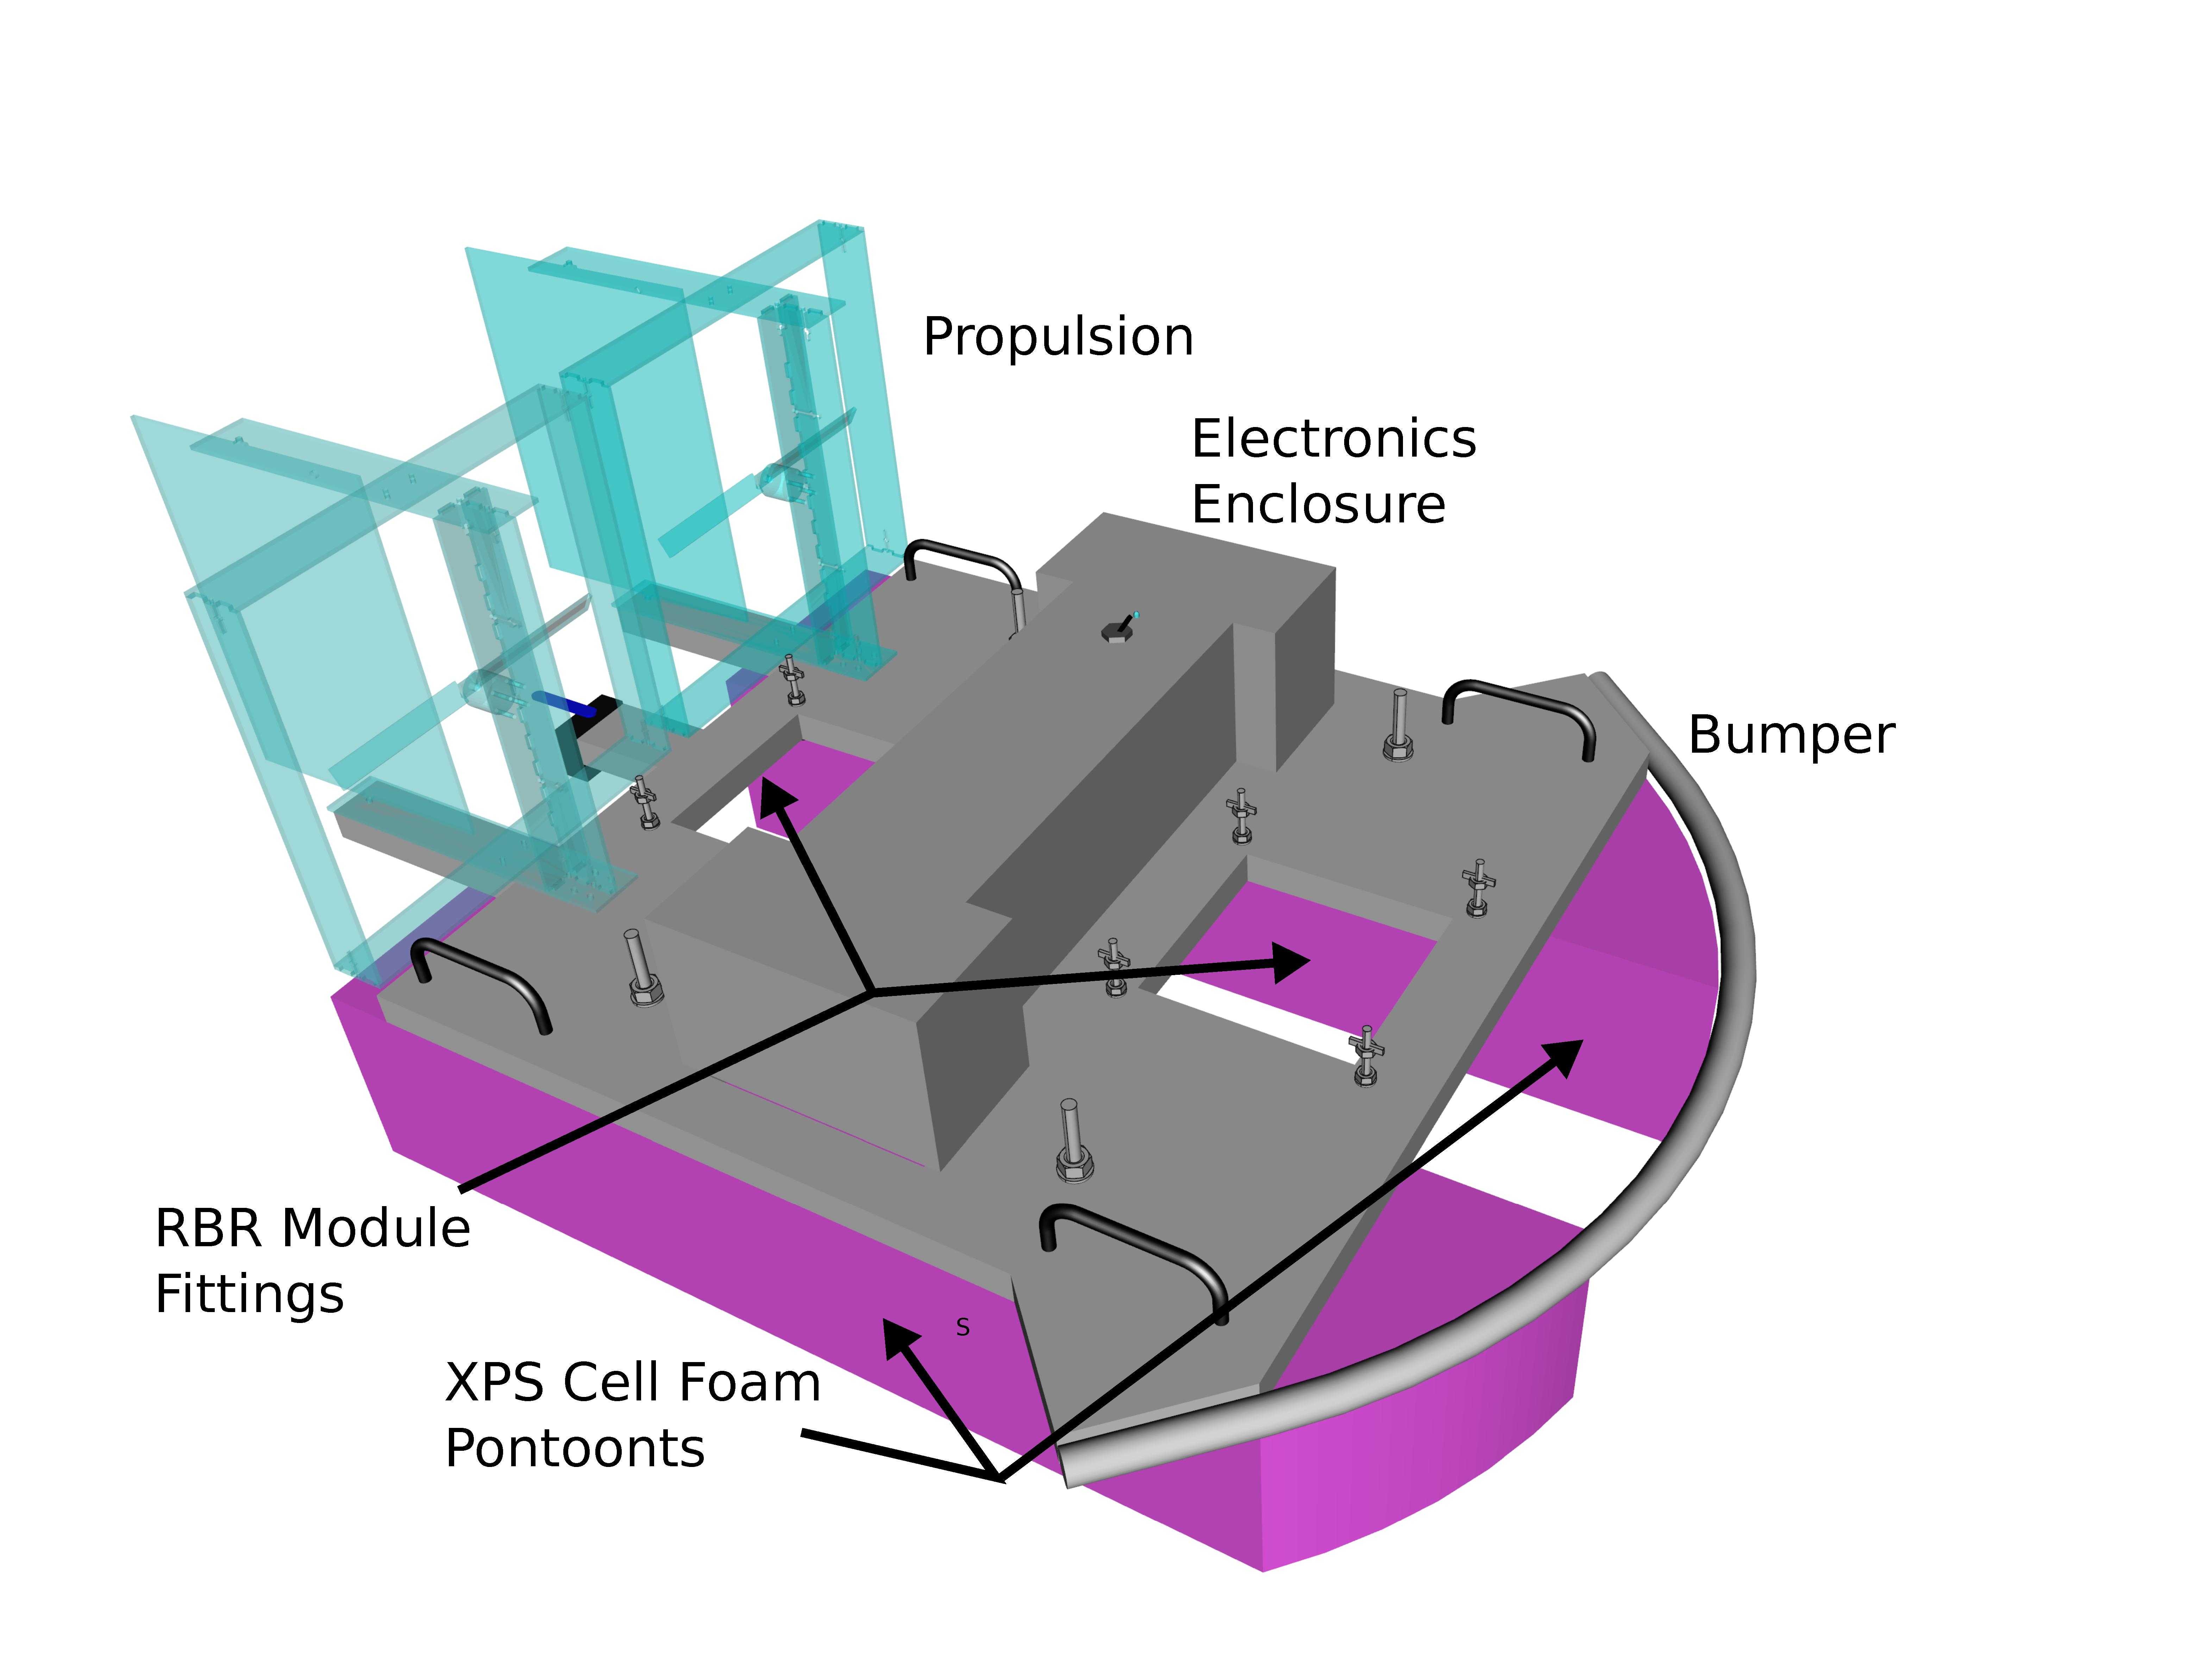
\includegraphics[width=.75\textwidth]{platformWithNotes.eps}
   \caption{The floating platform without the RBR modules installed}
   \label{fig:floatingPlatform}
\end{figure}           

\subsection{RBR module}
The RBR module consists of two baffles, separated by three adjustable threaded rods. The upper mounted baffle has a modified hand-held screwdriver attached on it, which is used to attach and drive a RBR with a shaft. The lower mounted baffle a PTFE shaft guide for a RBR axle. The lower mounted baffle also has an additional baffle that goes down into the water just above where a mounted RBR will be. This is so that no large vortices will be created above the RBR. 

The upper baffle can be adjusted hight wise in order to problem dial in the depth in which a RBR will work. Usually it's enough if the RBR are on the a depth so it just passes the pontoons of the floating platform.

The speed of the RBRs can be controlled remotly through the radio controller from a low speed to up about 600 rpm on its maximum setting. Around 500 rpm is ideal, then the RBR can do its work well at the same time as the battery drain is as small as possible. 

To attach the module to the platform, it is positioned in one of the the intended slots and attached with four fly nuts and wired up to the main power supply described in the electronics section.

\subsection{Propulsion}
The propulsion is made from air-propellers installed in a acrylic plastic protection housing. In order to be able to turn, rudders have been installed in front of the propellers. These are controlled through a single servo in the back of the floating platform. The layout of the propulsion mechanism is depicted in figure . Due to the material it has been made out of the propulsion mechanism can be delicate, so care when transporting is advised. 
\begin{figure}[h]
   \centering
   \includegraphics[width=.75\textwidth]{circuit}
   \caption{The propulsion construction}
   \label{fig:circuit}
\end{figure}

\subsection{Water protection}
To protect the RBR module drive assembly, the batteries, engine control units, and other electronic equipment, acrylic protection covers were manufactured. These does not protect the equipment from submersion, only from small splashes or rain. 
\subsection{Transportation}
To ease transportation, the weight of the platform can be decreased by first removing the power cables to the batteries, and RBR modules, both situated underneath the protective covers. The batteries and RBR modules can then be removed by releasing the battery straps and module fly nuts which allows for removing these components. Care needs to be taken such that the propulsion mounts are not damaged during transport, as these parts are fragile.


\clearpage
\section{Radio Controller}
The radio controller, used to steer the boat, is a Radiolink AT9 9 channel 2.4GHz control system. The controller supports the provided Radiolink R9D receiver which is a 9 channel, 2.4 GHz DSSS (Direct-sequence spread spectrum) receiver.
\subsection{Steering}
The Layout of the buttons on the controller can be seen in Figure \ref{fig:controller_front}, and \ref{fig:controller_back} for the front, and back of the controller respectively. In Figure \ref{fig:controller_front} the \textit{Rudder/Elevator stick} is used to control the speed of propellers driving the boat forward. The propellers will be still when the stick is in the lowest position in the figure, and will have max speed when the stick is in the top most position in the figure. Note that the stick should be put in the lowest position when the electronics of the boat is powered on.

The \textit{Throttle/Aileron Stick} is used to control the air rudder. Moving the stick to the right will turn the boat to the right and moving it to the left will turn the boat left.

The stick on the back of the controller, the \textit{VRC SW} stick in Figure \ref{fig:controller_back} is used to control the rotational speed of the RBRs. If the stick is in the bottom most position the RBRs will not rotate. By moving the stick upwards the speed will increase until the stick is in the top position.
% Latexkod för bilderna jag lagt i denna mapp
\begin{figure}[h]
   \centering
   \includegraphics[width=.75\textwidth]{controller_front}
   \caption{The front of the radio controller and its buttons.}
   \label{fig:controller_front}
\end{figure}
\begin{figure}[h]
   \centering
   \includegraphics[width=.75\textwidth]{controller_back}
   \caption{The back of the radio controller and its buttons.}
   \label{fig:controller_back}
\end{figure}

\subsection{Settings}
When it comes to the settings in the controlled we used the base settings of the Helicopter type, which can be found under \textit{Model sel.} in the basic menu of the controller. The basic menu is found by holding in the \textit{mode} button. Some settings however were changed to be able to maneuver the vehicle more easily. The first of these setting tweaks were to put channel 1-3 from normal to reversed, in order to get the buttons to behave in a way better suited for a boat. This is done in \textit{reverse}, which can be found in the Basic menu. In order to get the \textit{VrC SW} button on the back of the controller, used to control the rotational speed of the RBRs (see Figure \ref{fig:controller_back} for button layout), one has to go into \textit{AUX-CH} in the basic menu and choose which channel  one want to couple it with. Then select \textit{VrC} on that channel. We chose to use channel 5 but any other channel can be used as well.

\clearpage
\section{Electronics}
\begin{figure}[p]
   \centering
   \includegraphics[width=.75\textwidth]{circuit}
   \caption{The circuit diagram of the electronics installed in floating platform}
   \label{fig:circuit}
\end{figure}

\clearpage
\section{Thoughts Behind Construction and Suggested Improvements}
\subsection{Floating Platform}
The initial design for the vehicle was a simple platform with two pontoons, one on either side, and that all other components would be mounted on top of this platform.  The pontoons are constructed from XPS cell foam, which is available in hardware and construction stores. The advantage of XPS over e.g. EPS foam, while more expensive, is that the material is denser and doesn’t absorb water. Cell foam is easy to form and work with, non-hazardous, and offers excellent buoyancy.

As the development progressed, the load that the platform would be required to bear was roughly estimated and served as a basis for the size of the pontoons. They were estimated to displace 20 kg with some margin to the water surface. The platform itself, constructed from glulam wood, was attached to the pontoons with 10 mm threaded rods. An advantage with wood is that it doesn’t sink, is recyclable, cheap, and easy to work with using simple tools. A disadvantage with wood is that it’s heavy. A hollow aluminium construction, e.g. sealed square tubing, could also be buoyant, and offer lighter weight. 

To distribute weight as evenly as possible, the RBR modules was placed at either end in the open space between the pontoons, and the rather heavy batteries were placed above the center of each pontoon. The batteries were placed in a slot in the platform to reduce weight, lower center of gravity and increase stability. The available space for electronics was thus limited to the middle of the platform, between the RBR modules.

To improve deflection of head on collisions, a rounded front bumper was added which also serves as a means of adding distance between the platform and any side obstacles. Without this bumper, the finished vehicle could be hard to manoeuvre out of tight spots.

\subsubsection{RBR modules}
To modularize the construction, we choosed that the RBRs should be self-contained with drive assembly and wave baffles in a module. This has the advantage of lowering the weight of the platform and reducing the transport dimensions. Beyond this the modularization gives the advantage that multipe RBR modules can be built and speed up the refill process when changing the cleansing material inside the RBR. If one has four RBR modules the unused modules can be preloaded and one only has to change the modules when refilling, maximizing the time the vehicle can spend cleaning the environment. It also allowed development and initial testing of the drive assembly and measurements of power consumption without a finished floating platform. 

On the top baffle of the RBR module we have attached a modified screwdriver to drive and attach a RBR with a shaft. The choice to use a screwdriver was to reduce cost, as it provides a suitably strong DC-motor together with a rugged chuck which is insensitive to off-axial loads (non-axial forces like roll forces, and forces from a not perfectly lined up construction). It also speeds up disassembly of the RBR axle from the drive assembly. Both baffles, with shaft guide and drive assembly is mounted above the surface, with only the RBR axle and RBR protruding below the surface. To reduce the formations of vortices induced by the rotation of the RBR, a wave baffle was mounted along the RBR axle to stop air from reaching the RBR.


\clearpage
\section{Material test - water purification}
In this study the capacity of different materials (concrete, zeolite, goethite,
ion exchange and activated carbon) to adsorb metal ions in polluted water over
time was investigated. The material were added in SpinChem\textsuperscript{\textregistered}'s rotating
bed reactors (RBR). The materials were sieved (300-700~$\mu$m) and washed in
deionized water before studied. The concentration of metal ions (copper and
zinc) was measured by the analytic methods FAAS and ICP-OES.

The spectro analytical method atomic absorption spectroscopy (AAS) determines the concentration of metal ions by taking up the solution in a heated flame, where the metal ions excites and absorb light that passes the flame specific for the metal ion.\cite{ford} The analytical technique inductively coupled plasma optical emission spectroscopy (ICP-OES) is used for measuring of the concentrations of metal ions. It produce excited atoms and ions by using the inductively coupled plasma at wavelength that is specific for a certain type of metal ion. The analytical methods has different detection limits depending on machine and metal ions, but in general ICP-OES can detect lower levels of metal ion concentration than FAAS. ICP-OES can also analyze several metal ions at the same measurement while FAAS can only analyze one metal ion at a time\cite{boss}\cite{fassel}. 

To measure metal ion concentration 20~ml material was added to the RBR~S221 in the SpinChem\textsuperscript{\textregistered} reaction vessel V211 contained 200~ml polluted water and rotated at 700~rpm during two time intervals. Before starting the stirrer motor, a reference sample was taken and then samples were taken during a time interval. In the first set, all materials were investigated separately and samples were taken three times: 30 minutes, 60 minutes and 120 minutes. The experiment was repeated for concrete, zeolites and goethite with time interval: 10~seconds, 1~minute, 3~minutes, 7~minutes, 15~minutes and 30~minutes. All samples were taken with a syringe and filtered into falcon tubes. To each ml sample, 10 $\mu$l 7~M nitric acid was added in the falcon tubes and sent to FAAS analysis. 

After the FAAS analysis, goethite was chosen for the ICP-OES analysis to further investigate its capacity to adsorb metal ions on a larger scale. 50~ml material was added to the RBR~S331 in the reaction vessel V311 contained $1.2$~l polluted water and rotated at 700~rpm. Nine samples including the reference sample were taken with a time interval: 0~minutes, 10~seconds, 1~minutes, 3~minutes, 7~minutes, 15~minutes, 30~minutes, 1~hour and 2~hours. All samples were taken with a syringe and filtered into falcon tubes. To each ml sample, 10~$\mu$ l 7~M nitric acid was added in the falcon tubes and analysed with ICP-OES. 

To examine how the material (concrete and goethite) affect pH during the reaction 20~ml material was added to the RBR S221 in the reaction vessel V211 contained 200~ml polluted water and rotated at 700~rpm. pH was measured with litmus paper during a two hour period (see \cref{tab:ph}). 

\subsection{Results}
The capacity of the different materials (concrete, zeolite, goethite, ion exchange and activated carbon) to adsorb metal ions in polluted water over time was analysed. The metal ions, zinc and copper, were measured with the analytic methods FAAS and ICP-OES.

The FAAS analysis for the concentration of zinc ions showed that the concentration of zinc ions decreased for all materials after 30 minutes (see \cref{image00}). The same reference sample was used for all the materials. Goethite was the material that decreased most after 120~minutes, while concrete was the material with the lowest adsorption capacity. Between 30~minutes and 120~minutes, the concentration of zinc ions increased with concrete as material. The FAAS analysis for the concentration of copper ions showed that the concentration of copper ions decreased for all materials except zeolites after 120 minutes (see \cref{fig:image01}). Between 60~minutes and 120~minutes, the concentration of copper ions increased for concrete.

\begin{figure}[H]
    \centering
    \includegraphics[width=0.7\textwidth]{image00}
    \caption{The concentrations of Zn$^{2+}$-ions in mg/l measured at four time
        points (0 min, 30 min, 60 min and 120 min) in five different materials
            (zeolites, goethite, active carbon, concrete and Amberlite resins)
            using the analytic method FAAS.}\label{fig:image00}
\end{figure}


\begin{figure}[H]
    \centering
    \includegraphics[width=0.7\textwidth]{image01}
    \caption{The concentrations of Cu$^{2+}$-ions in mg/l measured at four time
        points (0 min, 30 min, 60 min and 120 min) in five different materials
            (zeolites, goethite, active carbon, concrete and Amberlite resins)
            using FAAS analysis.}\label{fig:image01}
\end{figure}

The experiment was repeated for zeolites, concrete and goethite but with shorter time interval and more frequent sampling. The concentration of zinc ion was analysed with FAAS. After 10 seconds the concentration of zinc ions had increased for all materials (see \cref{fig:image02}). After 30 minutes, goethite was the material that had adsorb most zinc ions and with concrete as material, the concentration of zinc ions started to increase after 7 minutes.

\begin{figure}[H]
    \centering
    \includegraphics[width=0.7\textwidth]{image02}
    \caption{The concentrations of Zn$^{2+}$-ions in mg/l measured at seven time
        points (0 min, 10 s, 1 min, 3 min, 7 min, 15 min and 30 min) in three
            different materials (zeolites, concrete and goethite) using FAAS
            analysis.}\label{fig:image02}
\end{figure}

The result for the ICP-OES analysis with goethite showed that the concentration of copper ions decreased until 15~minutes and between 15~minutes and 120~minutes the concentration was stable at $0.02$~mg/l (\cref{fig:image03}). The result for the concentration of zinc ions with goethite displayed negative values but it seems to decrease until 3~minutes and then flatten out (\cref{fig:image04}).

\begin{figure}[H]
    \centering
    \includegraphics[width=0.7\textwidth]{image03}
    \caption{The concentration of Cu$^{2+}$-ions in mg/l measured at nine time
        points (0 s, 10 s, 1 min, 3 min, 7 min, 15 min, 30 min, 60 min and 120
                min) with goethite and analysed with ICP-OES.}\label{fig:image03}
\end{figure}


\begin{figure}[H]
    \centering
    \includegraphics[width=0.7\textwidth]{image04}
    \caption{The concentration of Zn$^{2+}$-ions in mg/l measured at nine time
        points (0 s, 10 s, 1 min, 3 min, 7 min, 15 min, 30 min, 60 min and 120
                min) with goethite and analysed with ICP-OES.}\label{fig:image04}
\end{figure}

The result for pH measurements of concrete and goethite in polluted water containing metal ions showed to be stable at pH~5 for goethite during the whole time interval (\cref{tab:ph}). For concrete, the pH rose from 5 to 10 the first 5~minutes and then raised to 12 until 120~minutes. 

\begin{table}[H]
\centering
\caption{pH measurements with litmus paper of concrete and goethite at eight
    time points (0 min, 5 min, 10 min, 15min, 30 min, 60 min, 90 min and 120
            min) in polluted water containing metal ions.}
\label{tab:ph}
\begin{tabular}{lllllllll}
minutes         & 0 & 5 & 10 & 15 & 30 & 60 & 90 & 120 \\
pH for concrete & 5 & 10 & 11 & 11 & 12 & 12 & 12 & 12 \\
pH for goethite & 5 & 5 & 5 & 5 & 5 & 5 & 5 & 5
\end{tabular}
\end{table}

\subsection{Discussion}
A part of this project was to use SpinChem\textsuperscript{\textregistered}'s RBR and evaluate the capacity of different materials to adsorb metal ions in solution over time. The results from the FAAS analysis showed that all materials adsorb zinc ions after 120 minutes but had different capacities (\cref{fig:image00}). The concentration of zinc ions in the solution decreased more during the first 30 minutes and then the levels were quite stable. This could be due to that the materials became saturated and was not able to adsorb more zinc ions. The results also showed that concrete seemed to leak out zinc ions back to the solution after 30~minutes. This might be because the bond between zinc ions and concrete is weak and unstable or it favors other ions in the solution. The results for copper ions showed that all materials except zeolites were able to adsorb first 30 minutes (\cref{fig:image01}). As for the materials to adsorb zinc ions the result showed a similar pattern and after 30~minutes the concentration of copper ions were quite stable. This could be due to that the materials became saturated and was not able to adsorb more copper ions. It seems like the zeolite is not able to adsorb copper ions and might has greater affinity for other ions. 

Since the result for zinc ions showed a large decrease the first 30~minutes for all material we chose to repeat the experiment with zeolite, concrete and goethite during a shorter time interval and with more time points. The result was unexpected because the concentration of zinc ions were quite unchanged during the 30 minutes (\cref{fig:image02}). This could be due to that the standard that has to be prepared for FAAS analysis was too high comparing to our samples and therefore no conclusion can be made from this result. 

After FAAS analysis we decided to continue the study with goethite since it had the highest capacity to adsorb zinc ions and copper ions (\crefrange{fig:image00}{fig:image01}{fig:image02}). We repeated the experiment in larger scale ($1.2$~l) and chose to analyse with ICP-OES. The result showed that the reduction of copper ions in solution decreased most first 15~minutes and then the concentration were quite stable at $0.02$ (\cref{fig:image03}). Goethite seems to become saturated after 15~minutes and therefore not able to adsorb more copper ions. The result for the concentration of zinc ions in solution showed negative values of the concentration but displayed a similar pattern as for copper ions (\cref{fig:image04}). Goethite seems to be able to adsorb copper ions the first 7~minutes and then become saturated. The negatively values can be due to some error of measurement in ICP-OES machine. 
The pH measurements for concrete and goethite gave different results. For goethite, the pH level was stable around 5 during the whole time interval (\cref{tab:ph}). This might be due to that the material bind to other ions or release ions that does not affect the pH. The pH raised from 5 to 12 the whole time range and the large increase of the pH could be that concrete leaked out ions that affected the pH. The material could also bind hydrogen ions that affect the pH. 

In summary, goethite seems to have best capacity to adsorb zinc ions and copper ions comparing with the other materials and concrete seems to leak out the metal ions after time. Since the concentration of metal ions was extremely low in the solution, already in the beginning, the analysis methods seemed not to be good enough as analytical tool for the study and in future a more sensitive method should be used. 

\clearpage
\section{Large scale test using a pH-indicator and sodium hydroxide}

\subsection{Background}
From the beginning it had been suggested by the company that a large scale test
with the finished product should take place. The test was first supposed to be
conducted with water resembling that of a mining pond with all of its usual
pollutants. The volume was set to be 20~m$^3$. In this volume, the raft should
maneuver its way, carrying one or more of their patterned reactors, loaded with
the material that performs best according to the experiments conducted during
the course of the project.  However after reconsideration, the company decided
it would be less wise to create 20 m$^3$ of heavy metal polluted water. In the
case that it could not be fully recovered, it would be both tedious and
expensive to dispose of. The volume decided was also deemed excessive and was
lowered to 2 m$^3$ instead.

\subsection{Method}
Instead of using polluted water it was suggested to create a pure visual test
using either a coloring called allura red and purify it by loading the reactor
chambers with active carbon (AC). This process colors the water red and when
the colored water passes through the reactor, the allura red would get adsorbed
by the AC, making it less and less red for every time a volume passes the
reactor. This process takes a considerable amount of time, but in return it has
the benefit of restoring the water to practically the same as it was before
staining it with allura red.

Or using the pH-indicator phenolftalein together with a base (NaOH) which would
dye the water pink when pH gets above~8. For the test with the phenolftalein
the reactor chambers would be loaded with cation-exchange (CER) resins
amberlight. The phenolftalein would be added to the 2~m$^3$ of water. This by
itself would not induce a coloring of the water, but when adding enough NaOH to
push the pH above 8-9 the phenolftalein would dye the water into a pink color.
The CER in the reactor chambers neutralizes the base until such that pH drops
below 8-9 and thereby decolor the water. This process would not require the
full volume of water to pass through the reactor, it would only require that
enough particles gets adsorbed to lower the pH below 8 in the whole volume.
The concerns for the IER test were the amounts of phenolftalein required to dye
the water, since the phenolftalein itself will not be adsorbed.

Compared to the AC process this method is very fast. However the water will not
be restored after decoloring it. Since the phenolftalein does not get adsorbed
itself, it is necessary to inspect whether or not phenolftalein would be ok to
dispose of in regular sewers. Turns out phenolftalien poses no danger as a
marine pollutant\todo{ref}, all the same it would be best to use as little as
possible.  Due to these facts it was decided that the large scale test would be
performed using the CER approach.

\subsection{Experimental set up}
A fixed volume of 150~ml distilled water, together with a fixed amount of
150~$\mu$l 1~M NaOH added for each run. A start concentration of phenolftalein
was set to 0.05~mg/l. For each new test that concentration was halved until the
pink coloring no longer appeared for the naked eye. The final concentration of
phenolftalien needed was a mere 0.78~percent of the start concentration. Scaled
up to the final volume of 2~m$^3$ it would only require 0.78~g of pure
phenolftalein. The final concentration would be 1.225~$\mu$M.
(\todo{ref} for calculations.)
With the known least amount of phenolftalein required the process of
minimizing the amount of NaOH needed could start. With a fixed amount of
phenolftalein (0.78~percent) in the same amount (150~ml) of distilled water,
1~Molar NaOH was added a few $\mu$l at a time until a pink color was visible.
Scaling up to the final volume of 2~m$^3$ revealed that it would require 3.5~L
of 1~M NaOH for the final test. (\todo{ref} for calculations.)

\subsection{Distilled vs. tapwater}
Since all of the minor tests had been performed using distilled water instead
of tapwater, which would be used in the large scale test, there was a need to
redo the previous experiments with tapwater. When testing the amounts of NaOH
needed, it seemed as though it required more NaOH the first run compared to the
rest of the runs. Since we did not want to waste phenolftalein, the same water
was used for the following test, the only differences were that a reactor
loaded with CER had been used to neutralize the NaOH in between. The theory
behind it is that the initial pH is lower than the pH where the pH-indicator
turns from pink to colorless. Meaning that for the first test the initial pH is
around 6-7 while the later tests starts at an initial pH of 8-9, thus requiring
smaller amounts of NaOH.  Comparing the initial pH between distilled water and
tapwater showed that distilled water had somewhat lower pH. After running the
CER loaded reactors without any added base there was a slight decrease in pH in
both the distilled water and tapwater. The decrease was however larger in
tapwater when comparing to the start pH value.  The new test showed that it
would require a small increase of phenolftalein from 0.78~g up to 1.17~g. The
NaOH was increased by a 10~fold.

\subsection{Scaling up}
When scaling up the project, testing in volumes of 5~L and 70~L it became clear
that the amount of base needed in order to visually detect a pink color
decreased exponentially. When testing with 70~L it only required 20~ml instead of
the expected 120~ml that was calculated from the 150~ml experiments. In the final
volume of 2~m$^3$ it only required 150~ml of 1~M NaOH to turn the entire volume
pink.  This can be explained by Lamberts law that explains that there is an
exponential correlation between the transmission of light through a substance,
the product of the absorption and the length the light passed through the
material.



\clearpage
\section{Compliance to specification}

The specification of requirements, which can be seen in Appendix \ref{kravspec}, outlined several objectives of this project. How well the requirements are fulfilled can be seen in \cref{tab:kravspec} below.

\FloatBarrier
\begin{table}[H]
\centering
\caption{The requirements shown in \cref{kravspec}, together with how well they are fulfilled}
\begin{tabular}{l p{0.28\linewidth} | l p{0.28\linewidth}}
\toprule
\rowcolor{lightgray}
Requirement & Compliance & Requirement & Compliance\\
\midrule
1 (a) &  Not tested but assumed to function properly. & 2 (e) &  It should be easy to implement a autonomous operating system. \\
\midrule
1 (b) &  The RBRs needed to be adjustable, and are also constructed in that fashion. & 2 (f) &  Not tested but assumed to not be fulfilled. \\
\midrule
1 (c) &  The constructed vehicle is 60x90 cm, this makes it larger than in the specifications. & 3 &  Most of the parts are easily replicable, and it should not be too hard to construct a new vehicle. \\
\midrule
2 (a) &  The vehicle is fuelled by electricity. & 4 &  The RBR modules are easy to remove from the platform, which makes it easy to change the cleaning material. \\
\midrule
2 (b) &  Can be manoeuvred with a radio controller.  & 5 (a)-(e) &  All listed materials have been tested and analysed. \\
\midrule
2 (c) &  No occurring problems when the RBRs are rotating. & 6 &  A successful test was performed, with the local newspaper filming. \\
\midrule
2 (d) &  Batteries are used, which can easily be removed and charged.  & 7 &  This objective was only partially completed, through video footage from different angles at the final tests. \\
\bottomrule
\end{tabular}
\label{tab:kravspec}
\end{table}
\clearpage

\appendix
\section{Materials and parts lists}\label{sec:appendix-a}

\subsection{Floating platform}

The floating platform is built up from the following parts:

\begin{itemize}
  \item 1 main plate made from 22~mm glulam wood. The front bumper,
    servo and containing straps for the batteries are screwed to this plate. (Blueprints in \cref{fig:appendix-blueprint-main-plate}.)
  \item 4 floating elements made from 70~mm XPS cell foam. (Blueprint in \cref{fig:appendix-blueprint-ponton}.)
  \item 2 boards that goes below the floating elements (Blueprint in \cref{fig:appendix-blueprint-ponton}.)
  \item 4 250~mm M10 stainless steel threaded rods
  \item 8 70~mm M6 stainless steel threaded rods
  \item 4 M10 nuts
  \item 4 M10 lock nuts
  \item 16 M6 nuts
  \item 8 M6 wing nuts
  \item 8 M10 washers
  \item A 20~mm plastic tube bent to a quarter circle with a radius of 400~mm
  \item 2 straps to keep the batteries in place
  \item 4 carry handles
  \item Self drilling screws and washers used to attach electronics, battery
    straps, and bumper.
\end{itemize}

\subsection{Electronics}
The electronic components mounted on the platform are:
\begin{itemize}
  \item 1 Arduino Leonardo
  \item 1 Dual VNH5019 Motor Driver Shield
  \item 2 2725 Brushless out-runner motors 1600~kv
  \item 2 ESC which matches the brushless motors
  \item 2 plastic propellers
  \item 1 15~kg servo
  \item 1 R9D Radio Control Receiver
  \item 1 blue power-LED (mounted on the cover)
  \item 1 220~$\Omega$ resistor
  \item 1 power switch (mounted on the cover)
  \item 1 0.1 $\mu$F capacitor rated for at least 12~V \footnote{\label{fotnot_app} These parts can be replaced with any suitable 12~V to 5~V power supply.}
  \item 1 22 $\mu$F capacitor rated for at least 5~V\textsuperscript{\ref{fotnot_app}}
  \item 1 L4940V5 linear regulator\textsuperscript{\ref{fotnot_app}}
  \item Protoboard for the 5~V PSU\textsuperscript{\ref{fotnot_app}} (See schematic \cref{fig:appendix-circuit-diagrams} in \cref{sec:appendix-b}.)
  \item A few meters unshielded mains cable 2x1.50~mm$^2$
  \item A few meters signal cable
  \item A few sensor cables and connectors (for servo, ESC, and power to RC receiver)
  \item Heat-shrink tubing to cover connections
  \item A few blade receptacle 4.8x0.5~mm fully insulated, blade terminal red
    4.8x0.8~mm, ring cable lug 4.3~mm used to connect the cables together.
  \item A few 2.54~mm pin headers for the connections to the Arduino.
\end{itemize}
 \Cref{fig:appendix-circuit-diagrams} in \cref{sec:appendix-b} shows the complete circuit diagram of these parts. The electronics are connected according to the circuit diagrams, and the files in \texttt{RBR\_driver.zip} is loaded onto the Arduino.

\subsection{RBR modules}
Each of the two RBR modules are built from the following parts:
\begin{itemize}
  \item 1 top plate made from a 22~mm glulam wood (\cref{fig:appendix-blueprint-rbr-module})
  \item 1 bottom plate made from a 22~mm thick board (\cref{fig:appendix-blueprint-rbr-module})
  \item 1 3D printed motor mount
  \item 1 motor, shuck, and gearbox taken from a Meec Tools 12~VDC cordless drill 
  \item 3 330~mm M10 stainless steel threaded rods
  \item 3 M10 locking nuts
  \item 9 M10 nuts
  \item 12 M10 washers
  \item 2 50~mm M4 stainless steel threaded rods
  \item 2 110~mm M4 stainless steel threaded rods
  \item 10 M4 washers
  \item 10 M4 nuts
  \item 4 long M3 screws
  \item 4 M3 nuts
  \item 4 M3 washers
  \item 1 shaft guide NS29
  \item 1 piece of 50~mm wide and 200~mm long piece of 2~mm stainless steel
    bent to form a baffle.
  \item 1 piece of metal to put pressure on top of the motor.
\end{itemize}

\subsection{Covers for RBR modules and electronics}
The cover for the RBR module are made from 5 pieces of 3~mm thick acrylic glass
glued together, with a handle attached on top. The blueprints for these are shown in
\cref{fig:appendix-blueprint-rbr-cover} and \cref{fig:appendix-blueprint-electronic-cover},
both in \cref{sec:appendix-b}.

The cover for the electronics are made from 13 pieces of 3~mm thick acrylic glass
glued together. On top of this cover the power switch is connected. This cover
was fastened to the platform using handmade angle brackets and a nut.

\clearpage
\section{Blueprints and schematics}\label{sec:appendix-b}
\subsection{Circuit diagrams}
\begin{figure}[H]
  \centering
  \includegraphics[width=0.7\textwidth]{Powersupply}
  \includegraphics[width=0.7\textwidth]{circuit}
  \caption{The circuit diagram for the electronics.}
  \label{fig:appendix-circuit-diagrams}
\end{figure}

\clearpage
\subsection{Covers}
\begin{figure}[H]
  \centering
  \raisebox{-\height}{ \includegraphics[scale=1]{RBR_cover}}
  \caption{Blueprint of the RBR cover in scale 1:2.}
  \label{fig:appendix-blueprint-rbr-cover}
\end{figure}

\begin{figure}[H]
  \centering
  \raisebox{-\height}{ \includegraphics[scale=1]{Electric_cover}}
  \caption{Blueprint of the electric cover in scale 1:5.}
  \label{fig:appendix-blueprint-electronic-cover}
\end{figure}

\clearpage
\subsection{Blueprints}
\begin{figure}[H]
  \centering
   \raisebox{-\height}{\includegraphics[scale=0.4]{RBR_mod_Top}}
   \raisebox{-1.02\height}{\includegraphics[scale=0.4]{RBR_mod_Bottom}}
  \caption{The top and bottom plates of the RBR module in scale 1:5}
  \label{fig:appendix-blueprint-rbr-module}
\end{figure}

\begin{figure}[H]
    \centering
    \includegraphics[scale=0.5]{mainPlate}
    \caption{The blueprint of the main plate in scale 1:10}
    \label{fig:appendix-blueprint-main-plate}
\end{figure}

\begin{figure}[H]
    \centering
    \raisebox{-\height}{ \includegraphics[scale=0.5]{ponton}}
    \raisebox{-1.1\height}{ \includegraphics[scale=0.5]{bottom_plank}}
    \caption{The blueprint of one ponton and the bottom board in scale 1:10}
    \label{fig:appendix-blueprint-ponton}
\end{figure}

\clearpage
\section{Specification of requirements}\label{kravspec}
.\todo{Jesper}


\end{document}

